\documentclass[preview]{standalone}

\usepackage{tikz}               % Diagrams

% Configuation
\usetikzlibrary{matrix}         % Use for diagram layout

\begin{document}
% Figure of numpy, scipy, matplotlib, pandas
\begin{figure}
  \centering
  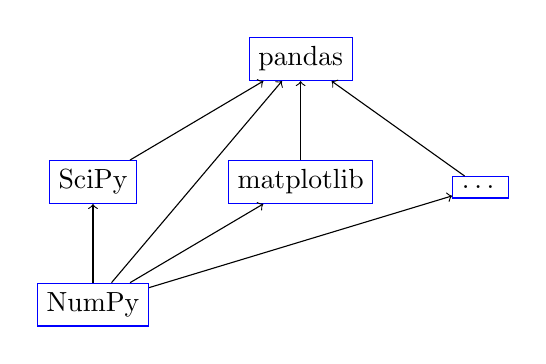
\begin{tikzpicture} [
    lib/.style={rectangle,draw=blue},
    ]
    \matrix [
    matrix of nodes,
    ampersand replacement=\&,
    row sep=10mm,
    column sep=10mm
    ] {
      % First row
      \&
      \node[lib] (pd) {pandas}; \&
      \\
      % Second row
      \node[lib] (sci) {SciPy}; \&
      \node[lib] (mpl) {matplotlib}; \&
      \node[lib] (etc) {\ldots}; \\
      % \footnote{statsmodels, pytables, sqlalchemy, python-dateutils, rpy;
      % libs for xml/html, spreadsheets.}}; \\
      % Third row
      \node[lib] (np) {NumPy}; \&
      \&
      \\
    };
    \path [<-]
    (pd) edge (sci) (pd) edge (mpl) (pd) edge (etc)
    (sci) edge (np) (mpl) edge (np) (etc) edge (np) (pd) edge (np);
  \end{tikzpicture}
  \caption{Dependencies of pandas for computation and plotting.}
\end{figure}
\end{document}
